\documentclass[a4paper,12pt]{article}

% Load Packages
\usepackage{amsfonts,amsthm,amsopn}
\usepackage[psamsfonts]{amssymb}
\usepackage[cmex10]{amsmath}
\usepackage{amsmath}
\usepackage{enumitem}
\usepackage{natbib}
\usepackage[left=3cm,right=3cm,top=3cm,bottom=3cm]{geometry}
\usepackage{xcolor}
\usepackage[]{graphicx}
\usepackage{graphics}
\usepackage{hyperref}
\usepackage[bb=dsserif]{mathalpha}
\usepackage{bm}
\usepackage{subcaption}

\newcommand{\ex}{\mathbb{E}}        % expectation
\newcommand{\bfbeta}{\bm{\beta}} %bold beta coefficent

\setlength\parindent{0pt}
\renewcommand{\baselinestretch}{1.2}



% Start document
\begin{document}



\begin{center}
\underline{\Large\textbf{{Reply to reports on article JBES-P-2022-0567}}}\end{center}
\vspace{10pt}


%First of all, we would like to thank the editor, the associate editor and the reviewers for their many comments and suggestions which were very helpful to improve the paper. In the revision, we have addressed all comments of the referees and have rewritten the paper accordingly. We also included an additional discussion of the extensions suggested by the referees that are closest to the original setup. Moreover, we have included additional details on the identification of the components in our multiplicative volatility model (cp. the beginning of Section 3.1) as we were not fully satisfied with the previous exposition.We also tweaked the simulation design to correspond more clearly to the setup discussed in the estimation section (cp. Section 7). 
%Finally, as requested, we have substantially shortened the paper to fit within the limit of 35 pages. This required to take all the proofs out of the paper and collect them in the supplementary material. In addition, we have rearranged the figures. In particular, the original Figures 2 and 3 are now contained in one figure. Similarly, the original Figures 6 and 7 are included in one figure. \\ 
%Please find our point-by-point responses to the referees below. In our responses, we have indicated where alterations to the manuscript have been made to account for the points raised. 



\subsection*{Reply to the editor}


\begin{enumerate}[label=\arabic*.,leftmargin=0.6cm]


\item \textit{The reviewers have diversified opinions, and they raise many issues. Although I think you can address many of them, there is one main issue I don’t see how to handle: As the AE points out, you do not have a compelling case for the null hypothesis that time trends are identical across multiple time series. Like the AE, I can’t think of different economic time series sharing the same trend.  I appreciate your discussions on clustering much more, but the same issue arises within a group. \\
There is a small econometric literature on co-trending and co-breaking where common time trends and breaks are used to capture comovements of multiple time series. Rather than time trends being identical, they are proportional to each other. That might be more plausible for modeling multiple economic time series. Because this may not be difficult in your framework, I do not mean to impose it.  Instead, I am pointing out that such literature may or may not be helpful. \\
Although I doubt the plausibility and usefulness of the null hypothesis, I would like to give the benefit of the doubt. I am willing to consider a revision of your paper, though with no guarantee that it will ultimately be accepted. I ask you to address all of the reviewers' concerns. Most importantly, please make a much more compelling and convincing case for the null hypothesis, which may be very difficult. I should note that this is not a typical R\&R and is a rather weak R\&R.
}


\end{enumerate}



\subsection*{Reply to the associate editor}


\begin{enumerate}[label=\arabic*.,leftmargin=0.6cm]


\item \textit{The less enthusiastic referee wrote: “Perhaps it is my unfamiliarity with the problem (or my tendencies toward Bayesian methodologies…), but I do not find it to be a particularly compelling research question. The goal is to test whether a time trend—after adjusting for covariates—is identical across multiple time series. This does not seem to be a high priority for multiple time series and dynamic regression analysis, and it’s not clear whether a hypothesis test generates much useful information in this context.” This is a comment I broadly agree with: would one really want/need to test for the exact “sameness” of time series trends? Or is it the case that the null hypothesis is uninteresting, but the alternative is, especially if I am able to see which trends are different and where? I am thinking aloud here, but overall I don’t think the testing problem, as stated, is interesting enough for JBES readers.}


\item \textit{There are two prior papers by the submitting author, which consider a similar problem but in the absence of external covariates. I don’t think the current paper makes it clear early enough what is different between the current work and those earlier papers.}  


\item \textit{Due to the various approximations, the size control is only approximate. I don’t see it as a ``state of the art'' way of thinking in these types of FWER control problems; please see e.g.\ \url{https://arxiv.org/abs/2009.05431},
where size control, in a different but related multiscale testing problem, is exact.}


\item \textit{I suspect the procedure must be really difficult to use in practice with confidence, as it depends on so many tuning parameters including the bandwidth. The authors say their software is at \url{https://github.com/marina-khi/multiscale_inference}, but the link is broken.}


\item \textit{ Both referees, including the more enthusiastic one, mention several further issues with the paper, including issues related to the practicalities of the method, the simulation study and the asymptotic nature of the method.}  

  
\end{enumerate}

  

\subsection*{Reply to referee 1}


Thank you very much for the careful reading of our manuscript and the interesting suggestions. In our revision, we have addressed all your comments. Please see our replies to them below.
\begin{enumerate}[label=\arabic*.,leftmargin=0.6cm]


\item \textit{The assumptions and requirements for the variance $\sigma^2$ deserve further consideration. First, it is claimed that the variances are assumed to be constant across series, but that a different estimator is used for each series. Which is the correct assumption for practice and theory? Second, given the economic and potential financial applications, how might volatility (or time-varying variance) be incorporated into the testing procedure? Is this plausible within the proposed framework, even if additional assumptions are required? If it is not plausible to account for volatility explicitly, then is the procedure robust in the presence of volatility? }


\item \textit{There are several issues with the simulation study. \\
(i) Setting the fixed effect to zero and including a single covariate both make for a much simpler design than considered in the theory. More challenging scenarios, including nonzero fixed effects and multiple predictors (e.g., using the estimated values and/or covariates from the application) would better demonstrate the capabilities of this approach. \\
(ii) The data from the null fix $m_i = 0$ and claim this is WLOG. However, this is also quite a simple case: the shared $m_i()$ curve could be quite complex under the null, which only maintains that the trends are shared among the series. \\
(iii) There are no competing methods considered; some alternative approach or benchmark must be added.  A reasonable alternative might consider an additive model and compute confidence intervals (or bands) for the trends, with a simple heuristic to determine whether the functions are identical. The proposed approach should do better, but demonstrating improvements over a reasonable alternative is important. \\
(iv) only a small number of series is considered. How does the approach perform when $n$ is large? }  

{\color{blue}  
In the simulation study, we need to take into account (i), (iii) and (iv). The point (ii) is not correct and can be taken care of by verbal argument.
\begin{itemize}[topsep=0pt]
 
\item[(i)] As we cannot use the estimated AR(1) values from the application, let's take the old simulation setup and modify it a bit {\color{red} (for the `robustness' check we also consider a case without any covariates, see the end of this section)}: 

\begin{itemize}[label=--,leftmargin=0.45cm,itemsep=0pt]

\item As before, we choose $n=15$ and $T=100,250,500$ {\color{red} (for an easy DGP without any covariates we use $T=100,250, 500, 750, 1000$. We also use this for comparison with SiZer in (iii).)}.
  
\item We include $3$ covariates and model them by a very simple VAR(3) process:
\[ \underbrace{\begin{pmatrix} X_{it,1} \\ X_{it,2} \\ X_{it,3} \end{pmatrix}}_{=: \boldsymbol{X}_{it}} = \begin{pmatrix} a_1 & 0 & 0 \\ 0 & a_2 & 0 \\ 0 & 0 & a_3 \end{pmatrix} \begin{pmatrix} X_{it-1,1} \\ X_{it-1,2} \\ X_{it-1,3} \end{pmatrix} + \underbrace{\begin{pmatrix} \nu_{it,1} \\ \nu_{it,2} \\ \nu_{it,3} \end{pmatrix}}_{=: \boldsymbol{\nu}_{it}}. \] 
We choose {\color{red} $a_1 = a_2 = a_3 = 0.25$}. The innovations $\boldsymbol{\nu}_{it}$ are drawn i.i.d.\ from a multivariate normal $N(0,\Phi)$ with
\[ \Phi = \begin{pmatrix} 1 & \varphi & \varphi \\ \varphi & 1 & \varphi \\ \varphi & \varphi & 1 \end{pmatrix}, \]
where $\varphi=0, 0.1, 0.25$ and setting $\varphi = 0$ results in simulating 3 independent covariate processes {\color{red}(case $\varphi = 0$ is not reported)}. 

\item We set $\boldsymbol{\beta}_i = (\beta_{i,1},\beta_{i,2},\beta_{i,3}) = (1,1,1)$ for all $i$.

{\color{red}\item We calculate the Gaussian quantiles based on $5000$ samples, and the size and power calculations are done based on $5000$ repetitions.}

\item As before, we assume that the errors $\varepsilon_{it}$ follow the AR(1) model $\varepsilon_{it} = a \varepsilon_{i(t-1)} + \eta_{it}$, where $a=0.25$ and the innovations $\eta_{it}$ are i.i.d.\ normal with zero mean $E[\eta_{it}]=0$ and variance $E[\eta_{it}^2]=0.25^2$ {\color{red}(setting higher variance results in lower signal-to-noise ratio and we are not hitting the size level)}. 

\item We let $\alpha = (\alpha_1,\ldots,\alpha_n)$ be a normally distributed random vector. In particular, $\alpha \sim N(0,c \Sigma)$ with
\[ \Sigma =
\begin{pmatrix}
1      & \rho   & \cdots & \rho   \\
\rho   & 1      & \ddots & \vdots \\
\vdots & \ddots & \ddots & \rho   \\
\rho   & \cdots & \rho   & 1
\end{pmatrix},
\]
where $\rho = 0.1, 0.25$ {\color{red}(larger values do not seem to affect the size that much)} gives the correlation across time series $i$. To start with, we set $c=1$ and then adjust it if needed.

\item To generate data under the null $H_0: m_1 = \ldots = m_n$, we let $m_i = 0$ for all $i$ as before. To produce data under the alternative, {\color{red}we use the bump functions $m_1(u) = b \cdot \mathbb{1}(u \in [0.3, 0.7]) \cdot \big(1 - \big\{\frac{u - 0.5}{0.2}\big\}^2\big)^2$ for $b = 0.25, 0.5, 1$ (depicted in Figure \ref{fig:bump_function}) and $m_i = 0$ for $i \neq 1$}. For the cluster analysis, it is presumably also better to use bump functions rather than linear maps. For example, we could use 3 groups with (scaled versions of) the functions $g_1$, $g_2$ and $g_4$ from Figure 2 in Vogt \& Linton (2020, Multiscale clustering of nonparametric regression curves).

\begin{figure}[t!]
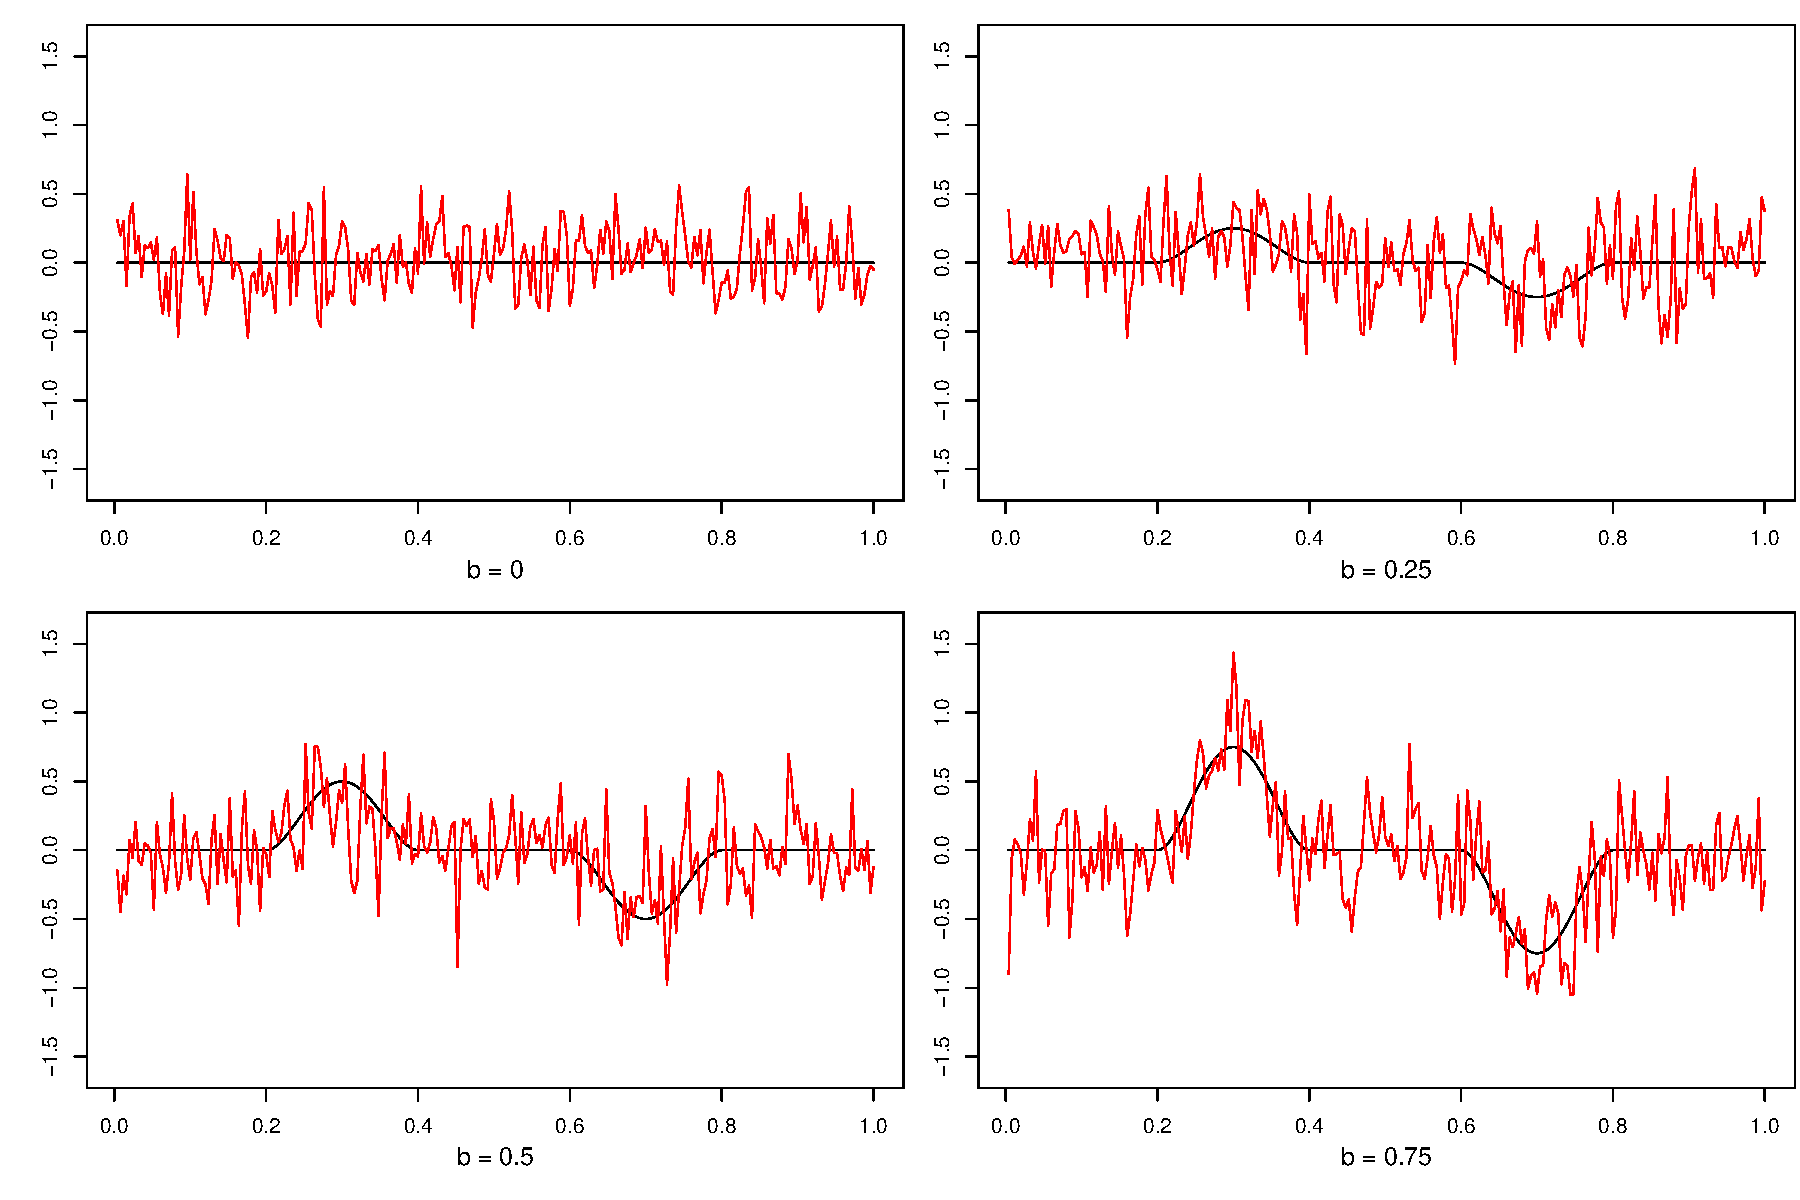
\includegraphics[width=\textwidth]{output/bump_function.pdf}
\caption{In black, the bump function $m_1(t/T)$ is plotted for different heights of the bump: $b = 0, 0.25, 0.5, 1$ ($b= 0$ corresponds to the data under the null $H_0$). In red, we depict the bump function plus the error term, $m_1(t/T) + \varepsilon_{it}$.}\label{fig:bump_function}
\end{figure}

\item We take the grid $\mathcal{G}_T$ to be the same as before: $\mathcal{G}_T = U_T \times H_T$, where $U_T = \big\{ u \in [0,1]: u = \textstyle{\frac{5t}{T}} \text{ for some } t \in \mathbb{N} \big\}$ and $H_T = \big\{ h \in \big[ \textstyle{\frac{\log T}{T}}, \textstyle{\frac{1}{4}} \big]:  h = \textstyle{\frac{5t - 3}{T}} \text{ for some } t \in \mathbb{N} \big\}$ {\color{red} (the grid is sparser for the DGP without any covariates: $\mathcal{G}_T = U_T \times H_T$, where $U_T = \big\{ u \in [0,1]: u = \textstyle{\frac{10t}{T}} \text{ for some } t \in \mathbb{N} \big\}$ and $H_T = \big\{ h \in \big[ \textstyle{\frac{\log T}{T}}, \textstyle{\frac{1}{4}} \big]:  h = \textstyle{\frac{5t - 3}{100}} \text{ for some } t \in \mathbb{N} \big\}$. Hence, the grid is growing only a bit with the sample size, because with the usual grid the actual size is still a bit higher than the nominal size even though the problem should be ``easy''. I guess this is because of the fact that with the growing sample size, the multiple testing problem becomes much more complicated... Moreover, the computational time is not feasible anymore for large values of $T$. )

\item In order to estimate the long-run variance $\sigma_i^2$, we follow the procedure described in \citet{KhismatullinaVogt2020} with the following tuning parameters: $q = 25$ and $r = 10$.
}

\end{itemize}

{\color{red} The results of the simulation study with the covariates are presented in Tables \ref{tab:size1} and \ref{tab:power1} for $\phi = 0.1$ and $\rho = 0.1$ and in Tables \ref{tab:size2} and \ref{tab:power2} for $\phi = 0.25$ and $\rho = 0.25$. We are a bit more liberal with higher values of $\phi$ and $\rho$, but not overly so. The results of the size simulation study without any covariates and for $\rho = 0.25$ are presented in Table \ref{tab:size3} (no power computations since this is more of a robustness check). There is a ``bump'' in the actual size for moderate sample sizes ($T = 250, 500$) which is present under a lot specifications (even without dependence in the fixed effect), I guess this is due to the grid specifications: for small sample size ($T = 100$) the grid is a bit too sparse to detect anything spurious, whereas starting from $T=250$ the grid becomes more sensitive to the noise which stabilizes with larger values of the sample size. I have checked with different grid specification and this ``bump'' is always present but occurs at different sample sizes.}

\begin{table}[t]
\footnotesize{
\begin{center}
\caption{Size of the multiscale test for $\phi = 0.1$ and $\rho = 0.1$ for different sample sizes $T$ and nominal sizes $\alpha$.}
\label{tab:size1}
\renewcommand{\arraystretch}{1.2}
% latex table generated in R 4.3.1 by xtable 1.8-4 package
% 
\begin{tabular}{cccc}
  \hline
  & \multicolumn{3}{c}{nominal size $\alpha$} \\
 $T$ & 0.01 & 0.05 & 0.1 \\
 \hline
100 & 0.010 & 0.040 & 0.083 \\ 
  250 & 0.021 & 0.078 & 0.132 \\ 
  500 & 0.019 & 0.067 & 0.127 \\ 
   \hline
\end{tabular}
%This simulation was done for the seed 1357913579, for the following values of the parameters: n_ts = 15, with 5000 simulations for calculating size and power and 5000 simulations to calculate the Gaussian quantiles. Furthermore, for the error process we have a = 0.25 and sigma = 0.25. For the covariate process a_1 = a_2 = a_3 = 0.25 and phi = 0.1. For the fixed effect, we have rho = 0.1. The grid is fine (growing with the sample size)

\end{center}}
\footnotesize{
\begin{center}
\caption{Power of the multiscale test for $\phi = 0.1$ and $\rho = 0.1$ for different sample sizes $T$ and nominal sizes $\alpha$. Each panel corresponds to a different height parameter $b$ of the bump function.}\label{tab:power1}
\begin{subtable}[b]{0.32\textwidth}
\centering
\caption{$b = 0.25$}\label{tab:power1_025}
\renewcommand{\arraystretch}{1.2}
% latex table generated in R 4.3.1 by xtable 1.8-4 package
% 
\begin{tabular}{cccc}
  \hline
  & \multicolumn{3}{c}{nominal size $\alpha$} \\
 $T$ & 0.01 & 0.05 & 0.1 \\
 \hline
100 & 0.012 & 0.051 & 0.098 \\ 
  250 & 0.138 & 0.314 & 0.446 \\ 
  500 & 0.567 & 0.767 & 0.853 \\ 
   \hline
\end{tabular}
%This simulation was done for the seed 1133557799, for the following values of the parameters: n_ts = 15, with 5000 simulations for calculating size and power and 5000 simulations to calculate the Gaussian quantiles. Furthermore, for the error process we have a = 0.25 and sigma = 0.25. For the covariate process a_1 = a_2 = a_3 = 0.25 and phi = 0.1. For the fixed effect, we have rho = 0.1. The grid is fine (growing with the sample size)

\end{subtable}
\begin{subtable}[b]{0.32\textwidth}
\centering
\caption{$b = 0.50$}\label{tab:power1_050}
\renewcommand{\arraystretch}{1.2}
% latex table generated in R 4.3.1 by xtable 1.8-4 package
% 
\begin{tabular}{cccc}
  \hline
  & \multicolumn{3}{c}{nominal size $\alpha$} \\
 $T$ & 0.01 & 0.05 & 0.1 \\
 \hline
100 & 0.011 & 0.053 & 0.094 \\ 
  250 & 0.865 & 0.954 & 0.980 \\ 
  500 & 1.000 & 1.000 & 1.000 \\ 
   \hline
\end{tabular}
%This simulation was done for the seed 22446688, for the following values of the parameters: n_ts = 15, with 5000 simulations for calculating size and power and 5000 simulations to calculate the Gaussian quantiles. Furthermore, for the error process we have a = 0.25 and sigma = 0.25. For the covariate process a_1 = a_2 = a_3 = 0.25 and phi = 0.1. For the fixed effect, we have rho = 0.1. The grid is fine (growing with the sample size)

\end{subtable}
\begin{subtable}[b]{0.32\textwidth}
\centering
\caption{$b = 1.00$}\label{tab:power1_100}
\renewcommand{\arraystretch}{1.2}
% latex table generated in R 4.3.1 by xtable 1.8-4 package
% 
\begin{tabular}{cccc}
  \hline
  & \multicolumn{3}{c}{nominal size $\alpha$} \\
 $T$ & 0.01 & 0.05 & 0.1 \\
 \hline
100 & 0.012 & 0.060 & 0.114 \\ 
  250 & 1.000 & 1.000 & 1.000 \\ 
  500 & 1.000 & 1.000 & 1.000 \\ 
   \hline
\end{tabular}
%This simulation was done for the following values of the parameters: n_ts = 15, with 5000 simulations for calculating size and power and 5000 simulations to calculate the Gaussian quantiles. Furthermore, for the error process we have a = 0.25 and sigma = 0.25. For the covariate process a_1 = a_2 = a_3 = 0.25 and phi = 0.1. For the fixed effect, we have rho = 0.1. The grid is fine (growing with the sample size)

\end{subtable}
\end{center}}
\vspace{-0.4cm}
\end{table}

\addtocounter{table}{-1} 
\begin{table}[t]
\footnotesize{
\begin{center}
\caption{Size of the multiscale test for $\phi = 0.25$ and $\rho = 0.25$ for different sample sizes $T$ and nominal sizes $\alpha$.}
\label{tab:size2}
\renewcommand{\arraystretch}{1.2}
% latex table generated in R 4.3.1 by xtable 1.8-4 package
% 
\begin{tabular}{cccc}
  \hline
  & \multicolumn{3}{c}{nominal size $\alpha$} \\
 $T$ & 0.01 & 0.05 & 0.1 \\
 \hline
100 & 0.008 & 0.039 & 0.085 \\ 
  250 & 0.018 & 0.072 & 0.118 \\ 
  500 & 0.014 & 0.070 & 0.124 \\ 
   \hline
\end{tabular}
%This simulation was done for the seed 111333555, for the following values of the parameters: n_ts = 15, with 5000 simulations for calculating size and power and 5000 simulations to calculate the Gaussian quantiles. Furthermore, for the error process we have a = 0.25 and sigma = 0.25. For the covariate process a_1 = a_2 = a_3 = 0.25 and phi = 0.25. For the fixed effect, we have rho = 0.25. The grid is fine (growing with the sample size)

\end{center}}
\footnotesize{
\begin{center}
\caption{Power of the multiscale test for $\phi = 0.25$ and $\rho = 0.25$ for different sample sizes $T$ and nominal sizes $\alpha$. Each panel corresponds to a different height parameter $b$ of the bump function.}\label{tab:power2}
\begin{subtable}[b]{0.32\textwidth}
\centering
\caption{$b = 0.25$}\label{tab:power2_025}
\renewcommand{\arraystretch}{1.2}
% latex table generated in R 4.3.1 by xtable 1.8-4 package
% 
\begin{tabular}{cccc}
  \hline
  & \multicolumn{3}{c}{nominal size $\alpha$} \\
 $T$ & 0.01 & 0.05 & 0.1 \\
 \hline
100 & 0.013 & 0.056 & 0.109 \\ 
  250 & 0.054 & 0.156 & 0.250 \\ 
  500 & 0.157 & 0.373 & 0.497 \\ 
   \hline
\end{tabular}
%This simulation was done for the following values of the parameters: n_ts = 15, with 5000 simulations for calculating size and power and 5000 simulations to calculate the Gaussian quantiles. Furthermore, for the error process we have a = 0.25 and sigma = 0.25. For the covariate process a_1 = a_2 = a_3 = 0.25 and phi = 0.25. For the fixed effect, we have rho = 0.25. The grid is fine (growing with the sample size)

\end{subtable}
\begin{subtable}[b]{0.32\textwidth}
\centering
\caption{$b = 0.50$}\label{tab:power2_050}
\renewcommand{\arraystretch}{1.2}
% latex table generated in R 4.3.1 by xtable 1.8-4 package
% 
\begin{tabular}{cccc}
  \hline
  & \multicolumn{3}{c}{nominal size $\alpha$} \\
 $T$ & 0.01 & 0.05 & 0.1 \\
 \hline
100 & 0.012 & 0.051 & 0.101 \\ 
  250 & 0.844 & 0.955 & 0.980 \\ 
  500 & 1.000 & 1.000 & 1.000 \\ 
   \hline
\end{tabular}
%This simulation was done for the seed 22446688, for the following values of the parameters: n_ts = 15, with 5000 simulations for calculating size and power and 5000 simulations to calculate the Gaussian quantiles. Furthermore, for the error process we have a = 0.25 and sigma = 0.25. For the covariate process a_1 = a_2 = a_3 = 0.25 and phi = 0.25. For the fixed effect, we have rho = 0.25. The grid is fine (growing with the sample size)

\end{subtable}
\begin{subtable}[b]{0.32\textwidth}
\centering
%\caption{$b = 1.00$}\label{tab:power2_100}
%\renewcommand{\arraystretch}{1.2}
%% latex table generated in R 4.3.1 by xtable 1.8-4 package
% 
\begin{tabular}{cccc}
  \hline
  & \multicolumn{3}{c}{nominal size $\alpha$} \\
 $T$ & 0.01 & 0.05 & 0.1 \\
 \hline
100 & 0.010 & 0.055 & 0.132 \\ 
  250 & 1.000 & 1.000 & 1.000 \\ 
  500 & 1.000 & 1.000 & 1.000 \\ 
   \hline
\end{tabular}

\end{subtable}
\end{center}}
\vspace{-0.4cm}
\end{table}

\addtocounter{table}{-1} 
\begin{table}[t]
\footnotesize{
\begin{center}
\caption{Size of the multiscale test for the case without any covariates and $\rho = 0.25$ for different sample sizes $T$ and nominal sizes $\alpha$.}
\label{tab:size3}
\renewcommand{\arraystretch}{1.2}
% latex table generated in R 4.3.1 by xtable 1.8-4 package
% 
\begin{tabular}{cccc}
  \hline
  & \multicolumn{3}{c}{nominal size $\alpha$} \\
 $T$ & 0.01 & 0.05 & 0.1 \\
 \hline
100 & 0.004 & 0.030 & 0.069 \\ 
  250 & 0.015 & 0.072 & 0.131 \\ 
  500 & 0.013 & 0.065 & 0.122 \\ 
  750 & 0.017 & 0.063 & 0.122 \\ 
  1000 & 0.012 & 0.072 & 0.123 \\ 
   \hline
\end{tabular}
%This simulation was done for the seed 1357913579, for the following values of the parameters: n_ts = 15, with 5000 simulations for calculating size and power and 5000 simulations to calculate the Gaussian quantiles. Furthermore, for the error process we have a = 0.25 and sigma = 0.25. We do not have any covarites. For the fixed effect, we have rho = 0.25. The grid is fine (growing with the sample size)

\end{center}}
\vspace{-0.4cm}
\end{table}


\item[(iii)] As suggested by you, we compare with the Sizer method of Park et al.\ (2009). For the comparison, we could consider the design proposed in (i) without covariates and fixed effects (as these are not part of the model in Park et al.). I'd suggest to add the comparison to the supplement rather than to the main body of the text.

{\color{red}Currently running. Do I understand correctly that we are comparing both in terms of size and power?}

\item[(iv)] We rerun the simulations from (i) with a much smaller grid. This allows us to deal not only with $n=15$ but also with larger values of $n$: $n=25, 50, 100$. Specifically, we take the grid $\mathcal{G}_T$ to be a dyadic scheme (as in Wavelet analysis) with scales in the set 
\[ \mathcal{H}_T = \big\{ h = 2^k h_{\min} \text{ for } k=0,\ldots,K \big\}, \]  
where 
\[ h_{\min} = \frac{\lceil \log T \rceil}{T} \]
and $K$ is such that $2^K h_{\min} \le \frac{1}{4}$, i.e.,
\[ K \le \Big\lfloor \log\Big(\frac{T}{4 \lceil \log T \rceil }\Big) \Big\rfloor \frac{1}{\log(2)}, \]
and 
\begin{align*}
\mathcal{G}_T = \big\{ (u,h) \subseteq [0,1]: & \ (u,h) = ((2s+1) h, h) \text{ for } s = 0,\ldots,\Big\lfloor \frac{h^ {-1}-1}{2} \Big\rfloor \\ & \ \text{and } h \in \mathcal{H}_T \big\}.
\end{align*}
{\color{red} We rerun the simulations as specified in (i) (with the exception of the grid) for the case $\phi = 0.1$ and $\rho = 0.1$ with $T=100, 250, 500$ and different values of $n$: $n=15, 25, 50, 100$. (This is very feasible, even with $n = 100$ and $T = 500$ the running time is around 45 minutes for all size and power calculations). The results are presented in Tables \ref{tab:size:dyadic:15} - \ref{tab:power:dyadic:100}. The results are not very different from using the full grid: we are not even much more liberal. I attribute it to the ``simplicity'' of the problem: not that many multiple comparisons.}

%\addtocounter{table}{-1} 
\begin{table}[t]
\footnotesize{
\begin{center}
\caption{Size of the multiscale test for $n = 15$ for different sample sizes $T$ and nominal sizes $\alpha$ for the dyadic grid ($\phi = 0.1$ and $\rho = 0.1$).}
\label{tab:size:dyadic:15}
\renewcommand{\arraystretch}{1.2}
% latex table generated in R 4.3.1 by xtable 1.8-4 package
% 
\begin{tabular}{cccc}
  \hline
  & \multicolumn{3}{c}{nominal size $\alpha$} \\
 $T$ & 0.01 & 0.05 & 0.1 \\
 \hline
100 & 0.007 & 0.030 & 0.064 \\ 
  250 & 0.012 & 0.054 & 0.103 \\ 
  500 & 0.009 & 0.050 & 0.091 \\ 
  750 & 0.011 & 0.057 & 0.107 \\ 
  1000 & 0.009 & 0.053 & 0.103 \\ 
   \hline
\end{tabular}
%This simulation was done for the seed 13579135, for the following values of the parameters: n_ts = 15, with 5000 simulations for calculating size and power and 5000 simulations to calculate the Gaussian quantiles. Furthermore, for the error process we have a = 0.25 and sigma = 0.25. For the covariate process a_1 = a_2 = a_3 = 0.25 and phi = 0.1. For the fixed effect, we have rho = 0.1. The grid is DYADIC.

\end{center}}
\footnotesize{
\begin{center}
\caption{Power of the multiscale test for $n = 15$ for different sample sizes $T$ and nominal sizes $\alpha$ for the dyadic grid ($\phi = 0.1$ and $\rho = 0.1$). Each panel corresponds to a different height parameter $b$ of the bump function.}\label{tab:power:dyadic:15}
\begin{subtable}[b]{0.32\textwidth}
\centering
\caption{$b = 0.25$}%\label{tab:power1_025}
\renewcommand{\arraystretch}{1.2}
% latex table generated in R 4.3.1 by xtable 1.8-4 package
% 
\begin{tabular}{cccc}
  \hline
  & \multicolumn{3}{c}{nominal size $\alpha$} \\
 $T$ & 0.01 & 0.05 & 0.1 \\
 \hline
100 & 0.007 & 0.040 & 0.086 \\ 
  250 & 0.113 & 0.238 & 0.352 \\ 
  500 & 0.510 & 0.701 & 0.795 \\ 
   \hline
\end{tabular}

\end{subtable}
\begin{subtable}[b]{0.32\textwidth}
\centering
\caption{$b = 0.50$}%\label{tab:power1_050}
\renewcommand{\arraystretch}{1.2}
% latex table generated in R 4.3.1 by xtable 1.8-4 package
% 
\begin{tabular}{cccc}
  \hline
  & \multicolumn{3}{c}{nominal size $\alpha$} \\
 $T$ & 0.01 & 0.05 & 0.1 \\
 \hline
100 & 0.069 & 0.184 & 0.283 \\ 
  250 & 0.729 & 0.881 & 0.930 \\ 
  500 & 1.000 & 1.000 & 1.000 \\ 
  750 & 0.960 & 0.993 & 0.998 \\ 
  1000 & 1.000 & 1.000 & 1.000 \\ 
   \hline
\end{tabular}
%This simulation was done for the seed 13579135, for the following values of the parameters: n_ts = 15, with 5000 simulations for calculating size and power and 5000 simulations to calculate the Gaussian quantiles. Furthermore, for the error process we have a = 0.25 and sigma = 0.25. For the covariate process a_1 = a_2 = a_3 = 0.25 and phi = 0.1. For the fixed effect, we have rho = 0.1. The grid is DYADIC.

\end{subtable}
\begin{subtable}[b]{0.32\textwidth}
\centering
\caption{$b = 1.00$}%\label{tab:power1_100}
\renewcommand{\arraystretch}{1.2}
% latex table generated in R 4.3.1 by xtable 1.8-4 package
% 
\begin{tabular}{cccc}
  \hline
  & \multicolumn{3}{c}{nominal size $\alpha$} \\
 $T$ & 0.01 & 0.05 & 0.1 \\
 \hline
100 & 0.013 & 0.068 & 0.126 \\ 
  250 & 1.000 & 1.000 & 1.000 \\ 
  500 & 1.000 & 1.000 & 1.000 \\ 
   \hline
\end{tabular}
%This simulation was done for the seed 13579135, for the following values of the parameters: n_ts = 15, with 5000 simulations for calculating size and power and 5000 simulations to calculate the Gaussian quantiles. Furthermore, for the error process we have a = 0.25 and sigma = 0.25. For the covariate process a_1 = a_2 = a_3 = 0.25 and phi = 0.1. For the fixed effect, we have rho = 0.1. The grid is DYADIC.

\end{subtable}
\end{center}}
\vspace{-0.4cm}
\end{table}

\addtocounter{table}{-1} 
\begin{table}[h!]
\footnotesize{
\begin{center}
\caption{Size of the multiscale test for $n = 25$ for different sample sizes $T$ and nominal sizes $\alpha$ for the dyadic grid ($\phi = 0.1$ and $\rho = 0.1$).}
\label{tab:size:dyadic:25}
\renewcommand{\arraystretch}{1.2}
% latex table generated in R 4.3.1 by xtable 1.8-4 package
% 
\begin{tabular}{cccc}
  \hline
  & \multicolumn{3}{c}{nominal size $\alpha$} \\
 $T$ & 0.01 & 0.05 & 0.1 \\
 \hline
100 & 0.006 & 0.030 & 0.059 \\ 
  250 & 0.015 & 0.056 & 0.104 \\ 
  500 & 0.016 & 0.068 & 0.127 \\ 
  750 & 0.012 & 0.060 & 0.113 \\ 
  1000 & 0.011 & 0.057 & 0.120 \\ 
   \hline
\end{tabular}
%This simulation was done for the seed 13579135, for the following values of the parameters: n_ts = 25, with 5000 simulations for calculating size and power and 5000 simulations to calculate the Gaussian quantiles. Furthermore, for the error process we have a = 0.25 and sigma = 0.25. For the covariate process a_1 = a_2 = a_3 = 0.25 and phi = 0.1. For the fixed effect, we have rho = 0.1. The grid is DYADIC.

\end{center}}
\footnotesize{
\begin{center}
\caption{Power of the multiscale test for $n = 25$ for different sample sizes $T$ and nominal sizes $\alpha$ for the dyadic grid ($\phi = 0.1$ and $\rho = 0.1$). Each panel corresponds to a different height parameter $b$ of the bump function.}\label{tab:power:dyadic:25}
\begin{subtable}[b]{0.32\textwidth}
\centering
\caption{$b = 0.25$}%\label{tab:power1_025}
\renewcommand{\arraystretch}{1.2}
% latex table generated in R 4.3.1 by xtable 1.8-4 package
% 
\begin{tabular}{cccc}
  \hline
  & \multicolumn{3}{c}{nominal size $\alpha$} \\
 $T$ & 0.01 & 0.05 & 0.1 \\
 \hline
100 & 0.014 & 0.050 & 0.099 \\ 
  250 & 0.081 & 0.213 & 0.303 \\ 
  500 & 0.476 & 0.665 & 0.763 \\ 
   \hline
\end{tabular}
%This simulation was done for the seed 13579135, for the following values of the parameters: n_ts = 25, with 5000 simulations for calculating size and power and 5000 simulations to calculate the Gaussian quantiles. Furthermore, for the error process we have a = 0.25 and sigma = 0.25. For the covariate process a_1 = a_2 = a_3 = 0.25 and phi = 0.1. For the fixed effect, we have rho = 0.1. The grid is DYADIC.

\end{subtable}
\begin{subtable}[b]{0.32\textwidth}
\centering
\caption{$b = 0.50$}%\label{tab:power1_050}
\renewcommand{\arraystretch}{1.2}
% latex table generated in R 4.3.1 by xtable 1.8-4 package
% 
\begin{tabular}{cccc}
  \hline
  & \multicolumn{3}{c}{nominal size $\alpha$} \\
 $T$ & 0.01 & 0.05 & 0.1 \\
 \hline
100 & 0.049 & 0.143 & 0.234 \\ 
  250 & 0.705 & 0.870 & 0.921 \\ 
  500 & 1.000 & 1.000 & 1.000 \\ 
   \hline
\end{tabular}
%This simulation was done for the seed 13579135, for the following values of the parameters: n_ts = 25, with 5000 simulations for calculating size and power and 5000 simulations to calculate the Gaussian quantiles. Furthermore, for the error process we have a = 0.25 and sigma = 0.25. For the covariate process a_1 = a_2 = a_3 = 0.25 and phi = 0.1. For the fixed effect, we have rho = 0.1. The grid is DYADIC.

\end{subtable}
\begin{subtable}[b]{0.32\textwidth}
\centering
\caption{$b = 1.00$}%\label{tab:power1_100}
\renewcommand{\arraystretch}{1.2}
% latex table generated in R 4.3.1 by xtable 1.8-4 package
% 
\begin{tabular}{cccc}
  \hline
  & \multicolumn{3}{c}{nominal size $\alpha$} \\
 $T$ & 0.01 & 0.05 & 0.1 \\
 \hline
100 & 0.009 & 0.039 & 0.086 \\ 
  250 & 1.000 & 1.000 & 1.000 \\ 
  500 & 1.000 & 1.000 & 1.000 \\ 
  750 & 1.000 & 1.000 & 1.000 \\ 
  1000 & 1.000 & 1.000 & 1.000 \\ 
   \hline
\end{tabular}
%This simulation was done for the seed 13579135, for the following values of the parameters: n_ts = 25, with 5000 simulations for calculating size and power and 5000 simulations to calculate the Gaussian quantiles. Furthermore, for the error process we have a = 0.25 and sigma = 0.25. For the covariate process a_1 = a_2 = a_3 = 0.25 and phi = 0.1. For the fixed effect, we have rho = 0.1. The grid is DYADIC.

\end{subtable}
\end{center}}
\vspace{-0.4cm}
\end{table}

\addtocounter{table}{-1} 
\begin{table}[h]
\footnotesize{
\begin{center}
\caption{Size of the multiscale test for $n = 50$ for different sample sizes $T$ and nominal sizes $\alpha$ for the dyadic grid ($\phi = 0.1$ and $\rho = 0.1$).}
\label{tab:size:dyadic:50}
\renewcommand{\arraystretch}{1.2}
% latex table generated in R 4.3.1 by xtable 1.8-4 package
% 
\begin{tabular}{cccc}
  \hline
  & \multicolumn{3}{c}{nominal size $\alpha$} \\
 $T$ & 0.01 & 0.05 & 0.1 \\
 \hline
100 & 0.006 & 0.031 & 0.063 \\ 
  250 & 0.010 & 0.051 & 0.102 \\ 
  500 & 0.023 & 0.076 & 0.126 \\ 
   \hline
\end{tabular}
%This simulation was done for the seed 13579135, for the following values of the parameters: n_ts = 50, with 5000 simulations for calculating size and power and 5000 simulations to calculate the Gaussian quantiles. Furthermore, for the error process we have a = 0.25 and sigma = 0.25. For the covariate process a_1 = a_2 = a_3 = 0.25 and phi = 0.1. For the fixed effect, we have rho = 0.1. The grid is DYADIC.

\end{center}}
\footnotesize{
\begin{center}
\caption{Power of the multiscale test for $n = 50$ for different sample sizes $T$ and nominal sizes $\alpha$ for the dyadic grid ($\phi = 0.1$ and $\rho = 0.1$). Each panel corresponds to a different height parameter $b$ of the bump function.}\label{tab:power:dyadic:50}
\begin{subtable}[b]{0.32\textwidth}
\centering
\caption{$b = 0.25$}%\label{tab:power1_025}
\renewcommand{\arraystretch}{1.2}
% latex table generated in R 4.3.1 by xtable 1.8-4 package
% 
\begin{tabular}{cccc}
  \hline
  & \multicolumn{3}{c}{nominal size $\alpha$} \\
 $T$ & 0.01 & 0.05 & 0.1 \\
 \hline
100 & 0.008 & 0.044 & 0.078 \\ 
  250 & 0.078 & 0.193 & 0.290 \\ 
  500 & 0.440 & 0.621 & 0.754 \\ 
   \hline
\end{tabular}

\end{subtable}
\begin{subtable}[b]{0.32\textwidth}
\centering
\caption{$b = 0.50$}%\label{tab:power1_050}
\renewcommand{\arraystretch}{1.2}
% latex table generated in R 4.3.1 by xtable 1.8-4 package
% 
\begin{tabular}{cccc}
  \hline
  & \multicolumn{3}{c}{nominal size $\alpha$} \\
 $T$ & 0.01 & 0.05 & 0.1 \\
 \hline
100 & 0.026 & 0.102 & 0.179 \\ 
  250 & 0.680 & 0.836 & 0.895 \\ 
  500 & 0.999 & 1.000 & 1.000 \\ 
   \hline
\end{tabular}
%This simulation was done for the seed 13579135, for the following values of the parameters: n_ts = 50, with 5000 simulations for calculating size and power and 5000 simulations to calculate the Gaussian quantiles. Furthermore, for the error process we have a = 0.25 and sigma = 0.25. For the covariate process a_1 = a_2 = a_3 = 0.25 and phi = 0.1. For the fixed effect, we have rho = 0.1. The grid is DYADIC.

\end{subtable}
\begin{subtable}[b]{0.32\textwidth}
\centering
\caption{$b = 1.00$}%\label{tab:power1_100}
\renewcommand{\arraystretch}{1.2}
% latex table generated in R 4.3.1 by xtable 1.8-4 package
% 
\begin{tabular}{cccc}
  \hline
  & \multicolumn{3}{c}{nominal size $\alpha$} \\
 $T$ & 0.01 & 0.05 & 0.1 \\
 \hline
100 & 0.006 & 0.040 & 0.081 \\ 
  250 & 1.000 & 1.000 & 1.000 \\ 
  500 & 1.000 & 1.000 & 1.000 \\ 
   \hline
\end{tabular}
%This simulation was done for the seed 13579135, for the following values of the parameters: n_ts = 50, with 5000 simulations for calculating size and power and 5000 simulations to calculate the Gaussian quantiles. Furthermore, for the error process we have a = 0.25 and sigma = 0.25. For the covariate process a_1 = a_2 = a_3 = 0.25 and phi = 0.1. For the fixed effect, we have rho = 0.1. The grid is DYADIC.

\end{subtable}
\end{center}}
\vspace{-0.4cm}
\end{table}

\addtocounter{table}{-1} 
\begin{table}[h!]
\footnotesize{
\begin{center}
\caption{Size of the multiscale test for $n = 100$ for different sample sizes $T$ and nominal sizes $\alpha$ for the dyadic grid ($\phi = 0.1$ and $\rho = 0.1$).}
\label{tab:size:dyadic:100}
\renewcommand{\arraystretch}{1.2}
% latex table generated in R 4.3.1 by xtable 1.8-4 package
% 
\begin{tabular}{cccc}
  \hline
  & \multicolumn{3}{c}{nominal size $\alpha$} \\
 $T$ & 0.01 & 0.05 & 0.1 \\
 \hline
100 & 0.007 & 0.029 & 0.063 \\ 
  250 & 0.014 & 0.062 & 0.115 \\ 
  500 & 0.018 & 0.078 & 0.144 \\ 
  750 & 0.011 & 0.061 & 0.116 \\ 
  1000 & 0.011 & 0.054 & 0.116 \\ 
   \hline
\end{tabular}
%This simulation was done for the seed 13579135, for the following values of the parameters: n_ts = 100, with 5000 simulations for calculating size and power and 5000 simulations to calculate the Gaussian quantiles. Furthermore, for the error process we have a = 0.25 and sigma = 0.25. For the covariate process a_1 = a_2 = a_3 = 0.25 and phi = 0.1. For the fixed effect, we have rho = 0.1. The grid is DYADIC.

\end{center}}
\footnotesize{
\begin{center}
\caption{Power of the multiscale test for $n = 100$ for different sample sizes $T$ and nominal sizes $\alpha$ for the dyadic grid ($\phi = 0.1$ and $\rho = 0.1$). Each panel corresponds to a different height parameter $b$ of the bump function.}\label{tab:power:dyadic:100}
\begin{subtable}[b]{0.32\textwidth}
\centering
\caption{$b = 0.25$}%\label{tab:power1_025}
\renewcommand{\arraystretch}{1.2}
% latex table generated in R 4.3.1 by xtable 1.8-4 package
% 
\begin{tabular}{cccc}
  \hline
  & \multicolumn{3}{c}{nominal size $\alpha$} \\
 $T$ & 0.01 & 0.05 & 0.1 \\
 \hline
100 & 0.008 & 0.037 & 0.076 \\ 
  250 & 0.053 & 0.152 & 0.244 \\ 
  500 & 0.426 & 0.596 & 0.689 \\ 
   \hline
\end{tabular}
%This simulation was done for the seed 13579135, for the following values of the parameters: n_ts = 100, with 5000 simulations for calculating size and power and 5000 simulations to calculate the Gaussian quantiles. Furthermore, for the error process we have a = 0.25 and sigma = 0.25. For the covariate process a_1 = a_2 = a_3 = 0.25 and phi = 0.1. For the fixed effect, we have rho = 0.1. The grid is DYADIC.

\end{subtable}
\begin{subtable}[b]{0.32\textwidth}
\centering
\caption{$b = 0.50$}%\label{tab:power1_050}
\renewcommand{\arraystretch}{1.2}
% latex table generated in R 4.3.1 by xtable 1.8-4 package
% 
\begin{tabular}{cccc}
  \hline
  & \multicolumn{3}{c}{nominal size $\alpha$} \\
 $T$ & 0.01 & 0.05 & 0.1 \\
 \hline
100 & 0.021 & 0.079 & 0.148 \\ 
  250 & 0.677 & 0.812 & 0.875 \\ 
  500 & 1.000 & 1.000 & 1.000 \\ 
   \hline
\end{tabular}
%This simulation was done for the seed 2468022, for the following values of the parameters: n_ts = 100, with 5000 simulations for calculating size and power and 5000 simulations to calculate the Gaussian quantiles. Furthermore, for the error process we have a = 0.25 and sigma = 0.25. For the covariate process a_1 = a_2 = a_3 = 0.25 and phi = 0.1. For the fixed effect, we have rho = 0.1. The grid is DYADIC.

\end{subtable}
\begin{subtable}[b]{0.32\textwidth}
\centering
\caption{$b = 1.00$}%\label{tab:power1_100}
\renewcommand{\arraystretch}{1.2}
% latex table generated in R 4.3.1 by xtable 1.8-4 package
% 
\begin{tabular}{cccc}
  \hline
  & \multicolumn{3}{c}{nominal size $\alpha$} \\
 $T$ & 0.01 & 0.05 & 0.1 \\
 \hline
100 & 0.005 & 0.034 & 0.074 \\ 
  250 & 1.000 & 1.000 & 1.000 \\ 
  500 & 1.000 & 1.000 & 1.000 \\ 
   \hline
\end{tabular}
%This simulation was done for the seed 13579135, for the following values of the parameters: n_ts = 100, with 5000 simulations for calculating size and power and 5000 simulations to calculate the Gaussian quantiles. Furthermore, for the error process we have a = 0.25 and sigma = 0.25. For the covariate process a_1 = a_2 = a_3 = 0.25 and phi = 0.1. For the fixed effect, we have rho = 0.1. The grid is DYADIC.

\end{subtable}
\end{center}}
\vspace{-0.4cm}
\end{table}

%With $T=100$ and $n=50$, we would get
%\[ \# \Big( \mathcal{G}_T \cup \{(i,j): 1 \le i < j \le n \} \Big) \approx 22000 \]
%(provided that I did not make any errors in my calculation \dots). Is this still feasible for the simulations???
%(The problem is that we consider all pairwise comparisons $(i,j)$. We could also cut down on this. One may also point out the following: spp there are different groups of time series (e.g. European and Asian countries). Then one may not be interested in comparing all of them but one may only compare the time series of different groups (e.g. European with Asian countries), which reduces the number of comparisons.) 

%T <- 100
%hmin <- ceiling(log(T))/T
%K    <- floor(log(T/4/log(T)) / log(2))
%Kvec <- 0:K
%NB   <- ceiling(sum(1/2^Kvec) / 2 / hmin)
  
%(Alternatively: Point out that the theory is for fixed $n$ only. Thus, we cannot say anything theoretically about large $n$, which is why we think it is better not to consider large $n$ in the simulations.)
  
\end{itemize}
}



\item \textit{Similarly, there are many related clustering methods, including (Bayesian and non-Bayesian) methods for clustering functional data. The proposed approach is reasonable, yet should be placed in a broader context and evaluated against appropriate competitors.}

{\color{blue}  
I think we could use the following clustering procedure as a benchmark:
\begin{itemize}[label=--,leftmargin=0.45cm,itemsep=0pt,topsep=0pt]
\item Estimate the trends $m_i$ by a local linear estimator $\hat{m}_i$ with a fixed bandwidth (chosen adhoc).
\item Compute a simple distance measure $d_{ij}$ between $\hat{m}_i$ and $\hat{m}_j$, e.g.
\[ d_{ij} = \int_0^1 (\hat{m}_i(w) - \hat{m}_j(w))^2 dw. \]
\item Construct the following dissimilarity measure from these distances:
\[ \hat{\Delta}(S,S') = \max_{i \in S,j \in S'} d_{ij}. \]
\item Run a HAC algorithm with the computed dissimilarities. 
\end{itemize}

Our procedure can be regarded as a further development of this very simple and natural benchmark procedure. In particular: our procedure replaces the simple distance measure $d_{ij}$ by a more advanced multiscale distance measure and provides a way to estimate the number of clusters, which is not part of the simple benchmark procedure.

As the benchmark procedure does not provide an estimate of the number of clusters $K$, it is presumably best to compare our procedure with the benchmark for known $K$. 

}
  

\item \textit{A related Bayesian strategy is to use simultaneous band scores (simBaS) to assess whether a function differs from zero. This could be applied pairwise to the differences between functions to establish a Bayesian competitor to the proposed approach, and simply requires posterior draws from an analogous Bayesian model.}

{\color{blue}  
We may argue here that we use the benchmark discussed in the previous comment instead of the proposed Bayesian strategy because it is naturally linked to our approach. 
}

  
\item \textit{The application includes numerous tuning parameters (including kernels, intervals, etc.). Are the results robust to these choices? Further details are needed.}

{\color{blue}  
The tuning parameters are:
\begin{enumerate}[label=(\alph*),leftmargin=0.75cm,itemsep=0pt,topsep=0pt]
\item the grid $\mathcal{G}_T$
\item tuning parameters to estimate the error variances $\sigma_i^2$ 
\item the number of bootstrap samples $L$ to compute the Gaussian quantile
\item the kernel $K$.
\end{enumerate}
(Have I forgotten anything here?)
  
We should run robustness checks:
\begin{enumerate}[label=(\alph*),leftmargin=0.75cm,itemsep=0pt,topsep=0pt]
\item We should consider different grids $\mathcal{G}_T$. In the simulation study, we use $\mathcal{G}_T = U_T \times H_T$ with
\begin{align*}
U_T & = \big\{ u \in [0,1]: u = \textstyle{\frac{5t}{T}} \text{ for some } t \in \mathbb{N} \big\} \\
H_T & = \big\{ h \in \big[ \textstyle{\frac{\log T}{T}}, \textstyle{\frac{1}{4}} \big]:  h = \textstyle{\frac{5t - 3}{T}} \text{ for some } t \in \mathbb{N} \big\}.
\end{align*}
We could additionally consider a finer grid with, e.g.,
\begin{align*}
U_T & = \big\{ u \in [0,1]: u = \textstyle{\frac{t}{T}} \text{ for some } t \in \mathbb{N} \big\} \\
H_T & = \big\{ h \in \big[ \textstyle{\frac{\log T}{T}}, \textstyle{\frac{1}{4}} \big]:  h = \textstyle{\frac{t}{T}} \text{ for some } t \in \mathbb{N} \big\}
\end{align*}
and a sparser one with, e.g.,
\begin{align*}
U_T & = \big\{ u \in [0,1]: u = \textstyle{\frac{10t}{T}} \text{ for some } t \in \mathbb{N} \big\} \\
H_T & = \big\{ h \in \big[ \textstyle{\frac{\log T}{T}}, \textstyle{\frac{1}{4}} \big]:  h = \textstyle{\frac{10t - 3}{T}} \text{ for some } t \in \mathbb{N} \big\}.
\end{align*}
I guess it is enough to consider only $n=15$ and $T=100$ for the robustness check. But I guess we should consider both the null and the alternative(s). 
\item I don't know whether it is necessary to consider different tuning parameters for the estimation of the error variance. Maybe we could run the procedure with the true $\sigma^2 = \sigma_i^2$ as a benchmark. Ideally, we can then report that the results produced by the benchmark are very similar to those produced by the feasible algorithm with estimated $\sigma_i^2$. I guess this should be enough.
%(One can also point out here that our method works with different estimators, i.e., one can use one's favourite estimator.)
\item One may compute the Gaussian quantile with different values of $L$. I guess the results should be very similar.  
\item I think there is no need to try out different kernels $K$ as from nonparametrics it is well known that the kernel is not so important.
%Actually one can make the point that the kernel is kind of part of the grid. 
\end{enumerate}
}
  
  
\item \textit{The multiscale tests are designed to control the FWER. Why is that the right criterion for the types of applications in mind (compared to e.g., FDR)? Given that other reasonable choices exist, additional motivation for this objective is warranted.}


\item \textit{I'm wondering if there might be some clarification about the independence of $\varepsilon_{it}$ across series $i$. In particular, suppose the intercepts $\alpha_i$ were instead considered random, like in mixed modeling (or Bayesian inference). Then marginally, the ``new'' errors ($\alpha_i + \varepsilon_{it}$) would be dependent across series $i$. Similar reasoning might apply to the covariates. From this perspective, the class of models might be considered more general.}

  
\item \textit{It is claimed on p.6 that the mean function integrating to zero is ``required'' for identification of the intercept. I think this is a sufficient, not necessary, condition, since others might suffice.} 

  
\end{enumerate}



\subsection*{Reply to referee 2}


Thank you very much for the careful reading of our manuscript and the interesting suggestions. We have addressed all your comments in the revision. Please see our replies to them below.
\begin{enumerate}[label=\arabic*.,leftmargin=0.6cm]

  
\item \textit{Although you correctly cite Khismatullina and Vogt (2020, 2021) on which quite a bit of this new work seems to be based can you please summarize more in particular about the test proposed in Khismatullina and Vogt (2021, Journal of Econometrics), and explain where and how your proofs differ from that (e.g.\ by the complexity in needing to treat the covariates).}


\item \textit{As your results are of asymptotic nature, it would be good to discuss limitations -- even give an example where the procedure would cease to work.}  


\item \textit{Moreover, can you at least sketch out if by something like a Bootstrap procedure (cf.\ Zhang et al, 2012) more of the ``asymptotic flavour'' of your test/cluster procedure could be remedied?}


\item \textit{I am having a slight (finite sample) identification concern with (not only your) model(s) mixing deterministic (nonparametric) trends with covariate (and also error) structure which is allowed to be positively serially dependent, e.g.\ autoregressive (as in your examples): I think that for ``any'' fixed sample size it might always occur that the trajectory of a stochastic trend, an autoregressive process with roots relatively close to the unit circle, say, cannot be distinguished from the deterministic trend. Wouldn't that be potentially a problem for your (and any related) test procedure? As a follow-up on this, wouldn't you need (or to say it differently, wouldn't it be perhaps beneficial to add) some extra conditions on the nature of your covariates (and potentially also your errors $\varepsilon$?) to avoid this problem?}  


\item \textit{What about a naive competitor that is just based on the second derivative (= change of the slope parameters) rather than the distance based on the curves and the first derivative (as in your local linear estimator)? I believe that this could also work rather well on your economic example data in Figures 3--6? Maybe you can ``benchmark'' your procedure against such a simple competitor (as such a comparison is somewhat missing explicitly -- although you orally compare sometimes with Zhang et al (2012)).}


\item \textit{Can your proposed test procedure be considered somehow to be equivalent to constructing a uniform confidence region where you would need to control if two (or more curves) are within the same tube (not just pointwise)? If so, it would be perhaps interesting to explain the link, and why for your test procedure it is sufficient/adequate to control the ``familywise'' error (does this correspond to what one does for a ``uniform'' region?).}


\item \textit{How in all of this does the number of curves (larger than two) play a role, in practice, for correctly calibrating your test (as least asymptotically as possible)? On the other hand, do your results reflect the fact that obviously they depend on the number of time series (or rather the number of series where trends are different, a number that you would have access to in an oracle situation)?}


\item \textit{Here is a small series of remarks towards needing to choose $(u, h)$ -- an example for a practical choice is given in Section 7, only (a bit late): Your localised multiscale method requires to discretize the continuous $(u, h)$. I am wondering if the way to do this plays a role for the properties of the resulting practical procedure. Can you please also compare with wavelet-based multiscale methods which are based somehow on a ``built-in'' way of choosing the location-scale parameters $(u, h)$?}  


\item \textit{page 12, around equation (3.6): it took me a moment to understand that you are talking about the standard local linear estimator (of Fan and Gijbels) here, you might want to make this clearer.}


\item \textit{I understand the heuristics behind using the Gaussian version (3.12) of the test statistics in the ``idealised'' situation but what about the ``non-idealised'' situation of unknown variances $\sigma^ 2$ and unknown parameters $\beta$? Is the Gaussian-based MC simulation method still valid when you need to estimate those parameters?}  


\item \textit{Again about the choice of $(u, h)$: what happens with expressions (such as in equation (4.1)) which depend on $\max_{(u,h)}$ in practice where you have to discretize this $(u, h)$? I do not think that a maximum over a continuous location-scale parameter can be treated the same way as one over a discrete one? Does the choice of the grid $\mathcal{G}_T$ influence the results here, don't you need some (additional) conditions on the grid (its spacing etc)? This refers, e.g.\ to the simulation section 6, page 24 where -- in passing -- you might want to change the strange wording there where you say ``for some t in N'' and rather detail the specification of the grid in $t$ here as you do later in Section 7.}  


\item \textit{Section 7, page 41, lines 45-50: can you develop this conjecture a bit?}


\item \textit{You might want to add a Conclusion Section which could both serve to recall the difficulties encountered in treating the more general situation of more than two curves and the presence of
covariates, and also discuss some of the aforementioned points on Bootstrap alternatives or on potential competitors.}  


\item \textit{Develop more to which extent the second data application (in the Supplement) brings insights beyond the one of the first (and why you chose to present the first and not the second in the main body of the text).}


\item \textit{Supplement section page 15, line 49 -- a notational detail: should the first $o_p$ be $O_p$ if the $\rho_T = o(1/ \log(T))$ or vice versa?}  


\item \textit{It would be good to explain somewhere in the main body (Section 3 or 4?) the additional difficulties in proving the results in the presence of the covariates.}
  
  
\end{enumerate}


\vspace{10pt}
\bibliographystyle{ims}
{\small
\setlength{\bibsep}{0.55em}
\bibliography{bib}}

%
%
%\large\textbf{{Bibliography}}
%\renewcommand\refname{}
%\vspace{-40pt}
%
%\normalsize
%\begin{thebibliography}{10}
%%\bibitem[Bickel et~el.(1993)]{Bickel1993} Bickel, P., Klaassen, C., Ritov, Y.\ \& Wellner, J.\ (1993). \textit{Efficient and adaptive estimation for semiparametric models.} Johns Hopkins University Press.
%%\bibitem[Fan et~al.(2005)]{Fan2005} Fan, J.\ \& Jiang, J.\ (2005). Nonparametric inferences for additive models. \textit{Journal of the American Statistical Association} \textbf{100} 890--907. 
%%\bibitem[Fengler et~al.(2015)]{Fengler2015} Fengler, M.~R., Mammen, E.\ \& Vogt, M.\ (2015). Specification and structural break tests for additive models with applications to realized variance data. \textit{Journal of Econometrics} \textbf{188} 196--218. 
%%\bibitem[Hafner \& Linton(2010)]{Hafner2009} Hafner, C.\ \& Linton, O.\ (2010). Efficient estimation of a multivariate multiplicative volatility model. \textit{Journal of Econometrics} \textbf{159} 55-73.
%%\bibitem[Huang et~al.(2010)]{Huang2010} Huang, J., Horowitz, J.~L.\ \& Wei, F.\ (2010). Variable selection in nonparametric additive models. \textit{Annals of Statistics} \textbf{38} 2282--2313.
%%\bibitem[Ravikumar et~al.(2009)]{Ravikumar2009} Ravikumar, P., Lafferty, J., Liu H. \& Wasserman, L.\ (2009). Sparse additive models. \textit{Journal of the Royal Statistical Society: Series B} \textbf{71} 905--1054.
%%\bibitem[Vogt \& Walsh(2019)]{VogtWalsh2019} Vogt, M.\ \& Walsh, C.\ (2019). Estimating nonlinear additive models with nonstationarities and correlated errors. \textit{Scandinavian Journal of Statistics} \textbf{46} 160-199.
%\end{thebibliography}



\end{document}
